\section{Circuito objetivo con valores modificados (Caso 2)}

\subsection{Parámetros y método}
El circuito conserva la topología del filtro activo del Caso 1 y modifica sus componentes. La fuente de entrada es de 10 V AC con fase de $0^\circ$. El análisis se resolvió mediante el modelo MNA lineal del op-amp ideal implementado por el proyecto. El modelo impone corrientes de entrada nulas y $V(NP)=V(NM)$; no representa saturación ni límites de alimentación.

\begin{table}[H]
\centering
\begin{tabular}{ll}
\toprule
Parámetro & Valor \\
\midrule
Frecuencia de inicio y final & 10 Hz y 100 kHz \\
Tipo de barrido & Lineal, 300 puntos \\
Fuente $V_1$ & 10 V AC, $0^\circ$ \\
$C_1$, $C_2$ & 0.50 $\mu$F cada uno \\
$R_{G1}$, $R_A$ & 3 k$\Omega$ cada uno \\
$R_{G2}$, $R_B$ & 1.5 k$\Omega$ cada uno \\
Op-amp & Ideal lineal, formulación MNA del proyecto \\
\bottomrule
\end{tabular}
\caption{Parámetros del circuito objetivo modificado.}
\end{table}

\begin{figure}[H]
\centering
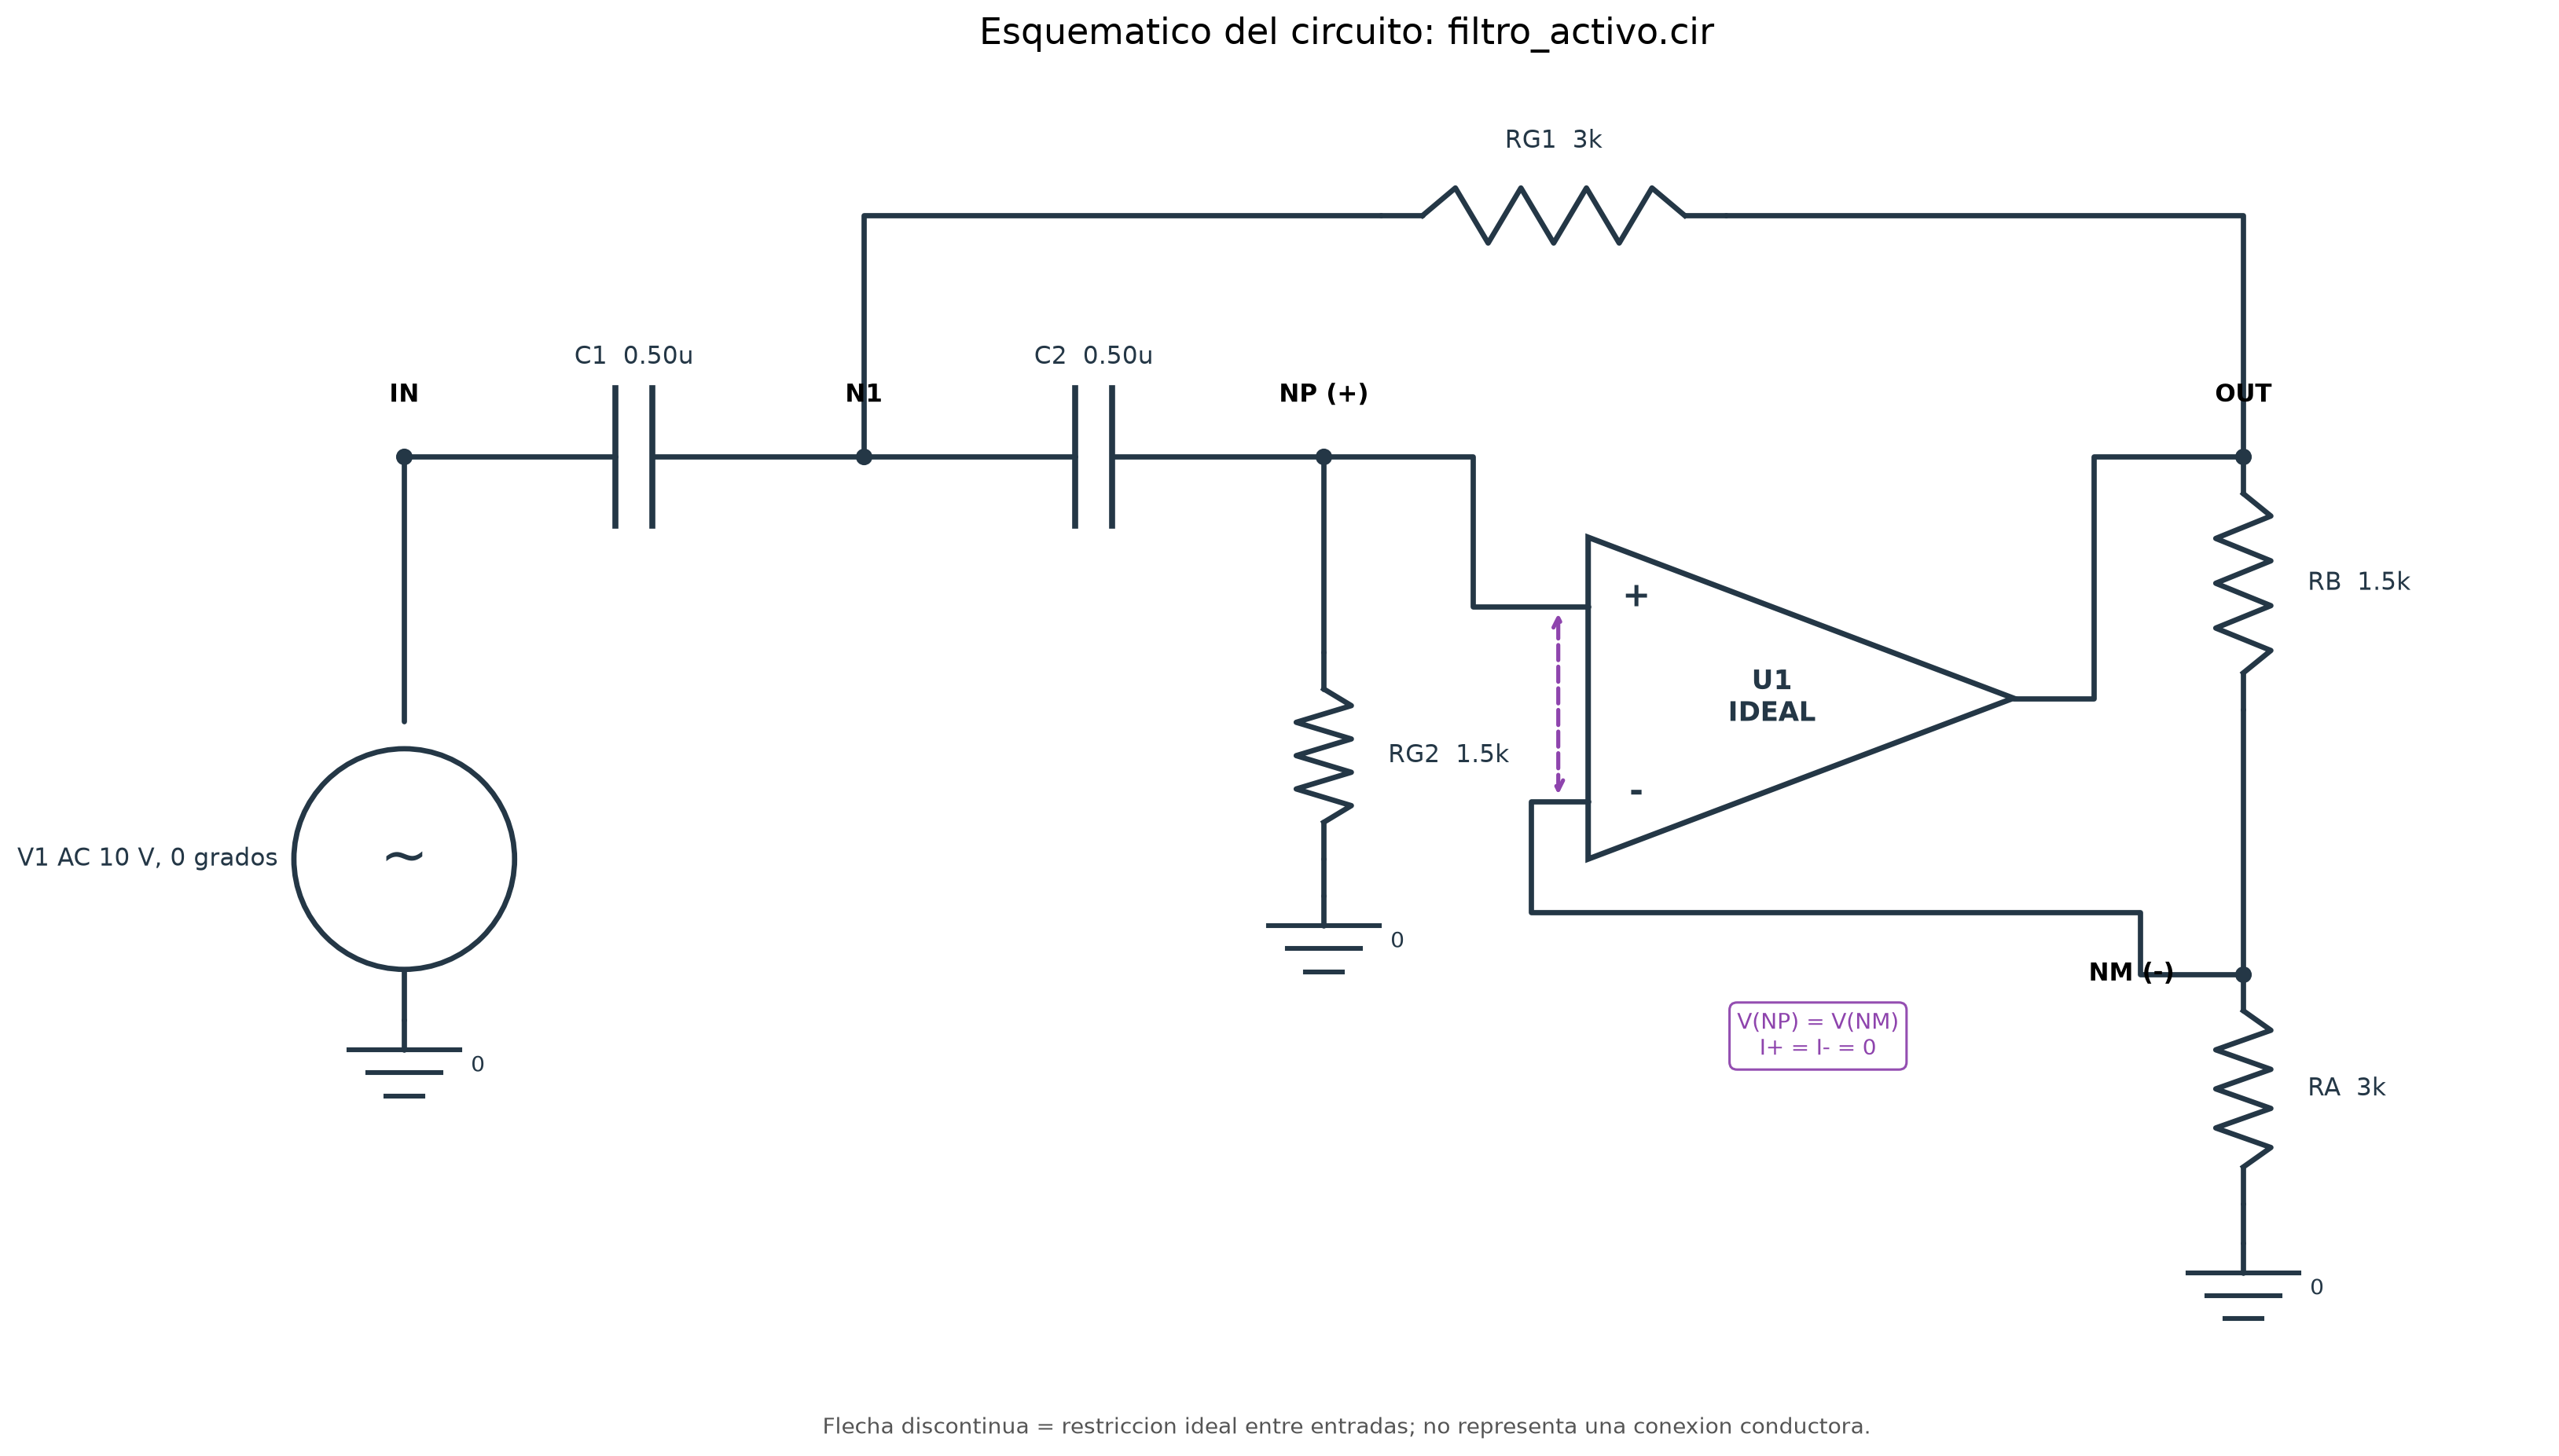
\includegraphics[width=0.78\linewidth]{2_circuito_objetivo_modificado_agent/plots/esquematico_filtro_activo.png}
\caption{Esquemático del filtro activo modificado.}
\end{figure}

\subsection{Topología y formulación}
La validación del netlist fue \textbf{Satisfactorio}. El análisis AC mediante MNA también fue \textbf{Satisfactorio}: 300 de 300 puntos fueron validados. La gráfica de topología conserva las conexiones del circuito; el op-amp ideal se representa mediante la restricción del modelo, no como una rama pasiva.

\begin{figure}[H]
\centering
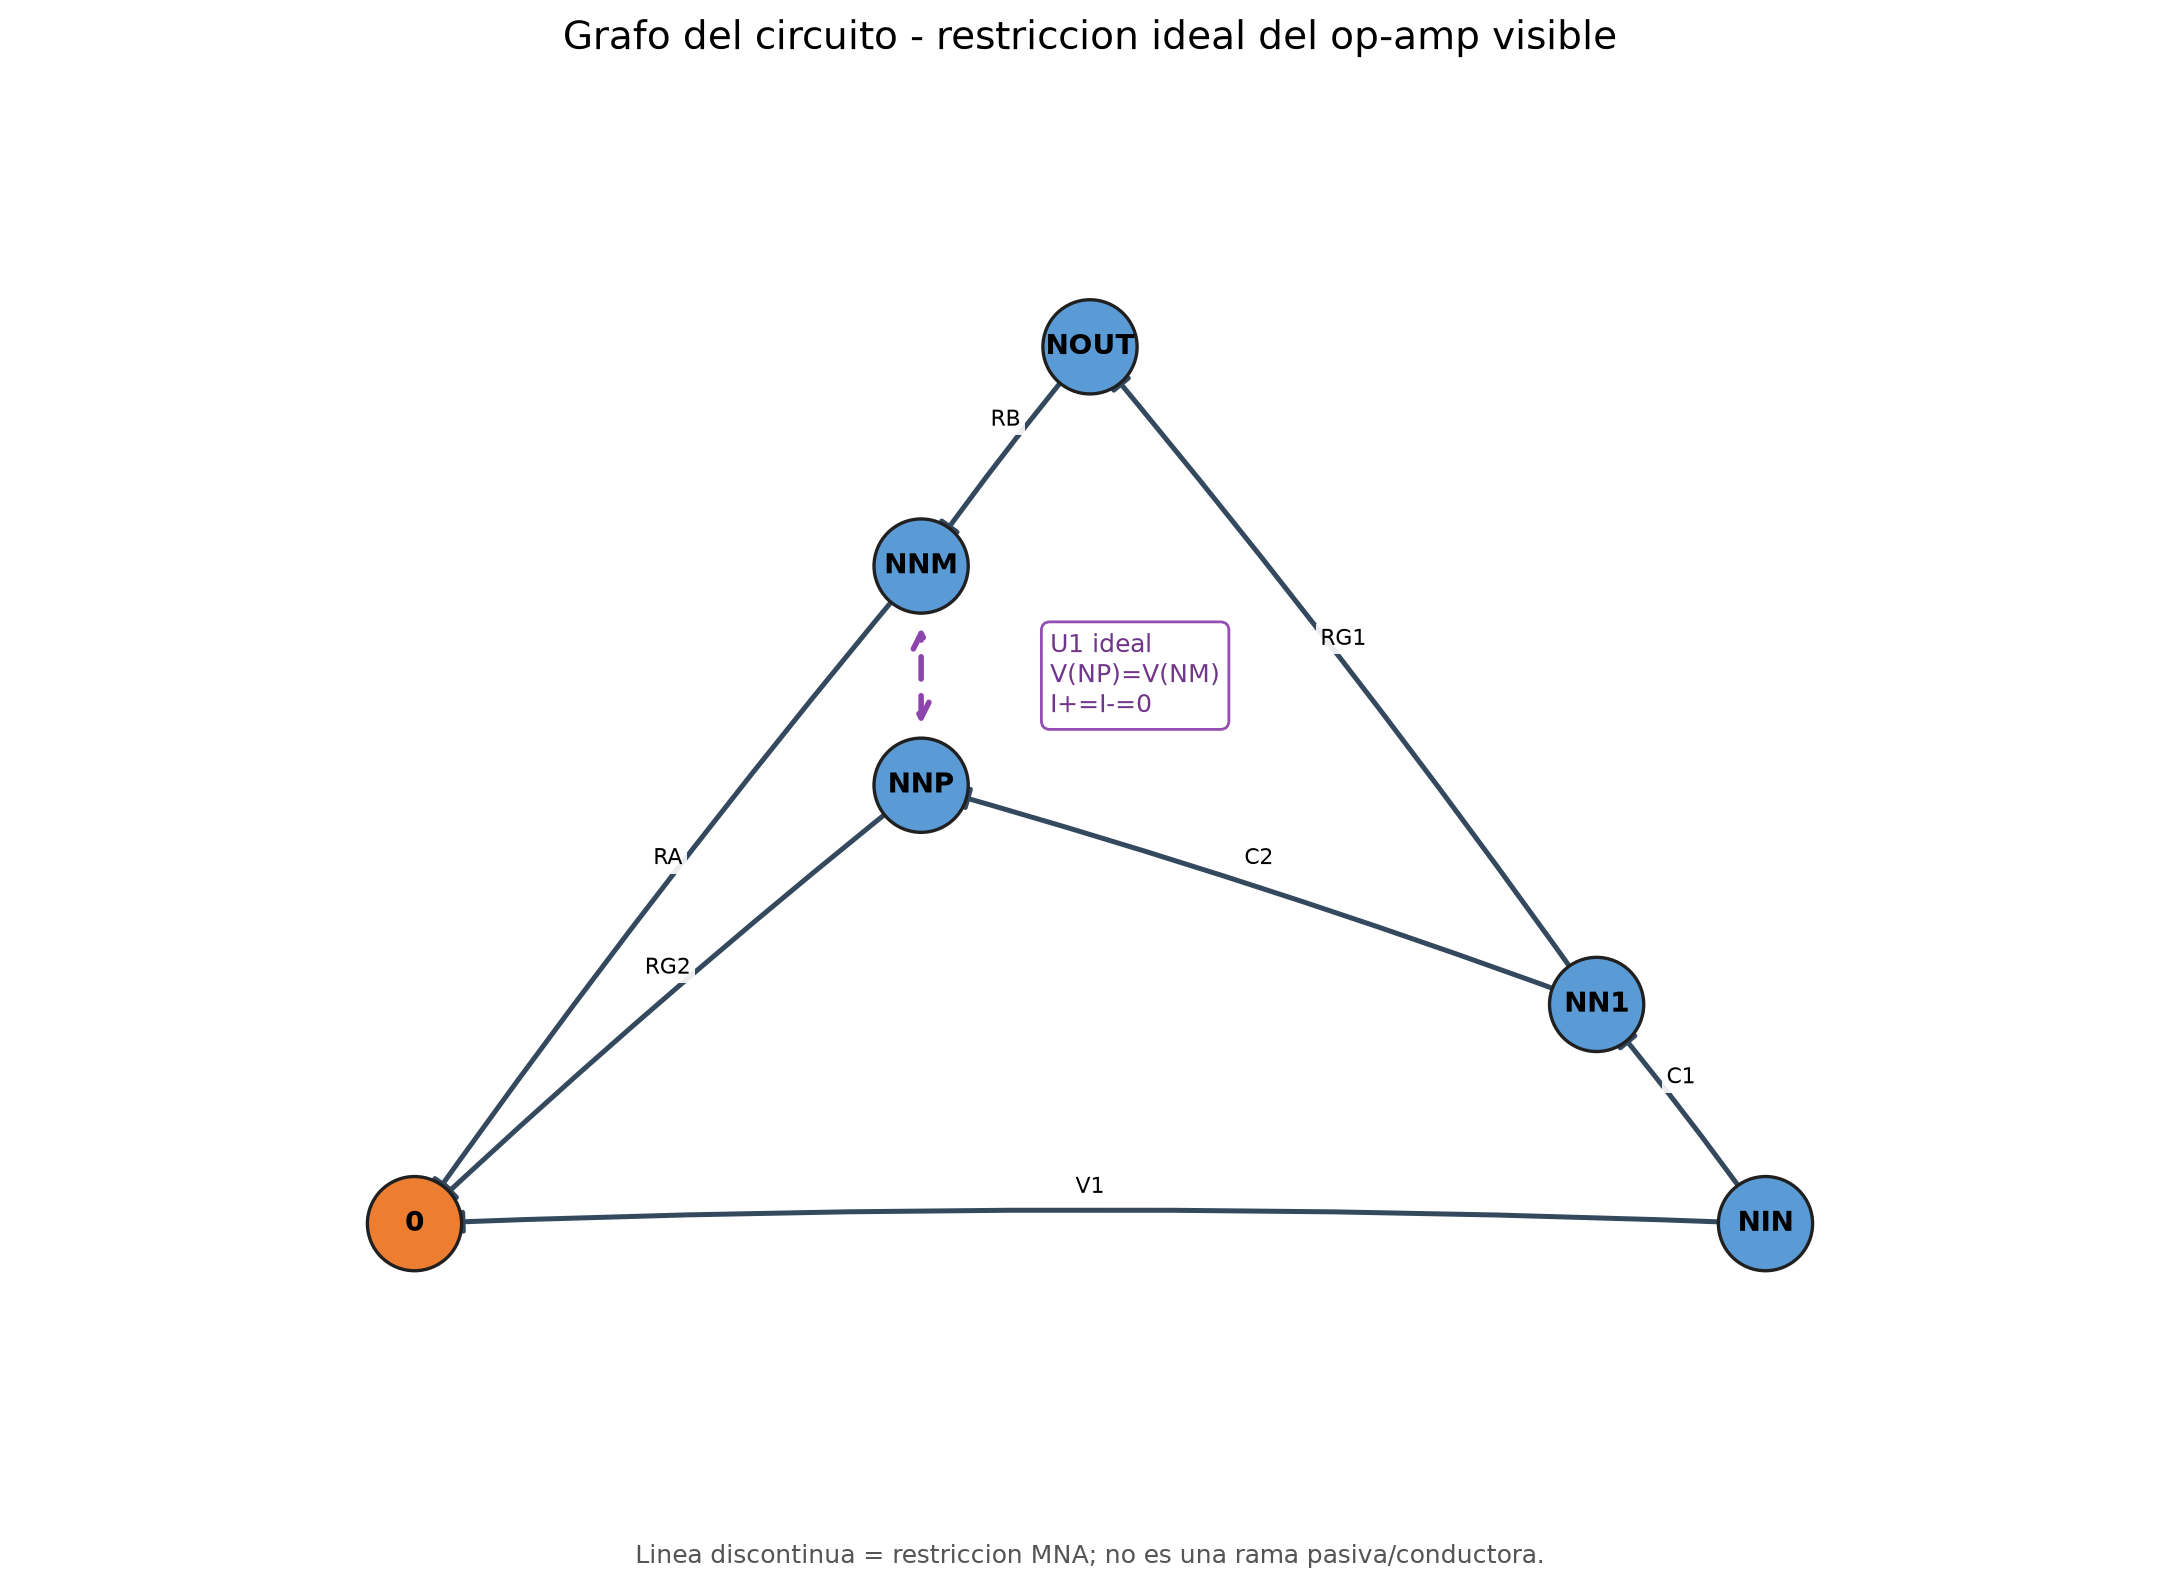
\includegraphics[width=0.78\linewidth]{2_circuito_objetivo_modificado_agent/plots/graph.png}
\caption{Grafo orientado del circuito modificado.}
\end{figure}

La matriz Tableau mostrada a continuación es \textbf{parcial}: se construye sin el bloque $U1$ y no resuelve el circuito completo. La solución válida del op-amp se obtiene con MNA; la matriz MNA completa a 10 Hz se incluye después.

\begin{figure}[H]
\centering
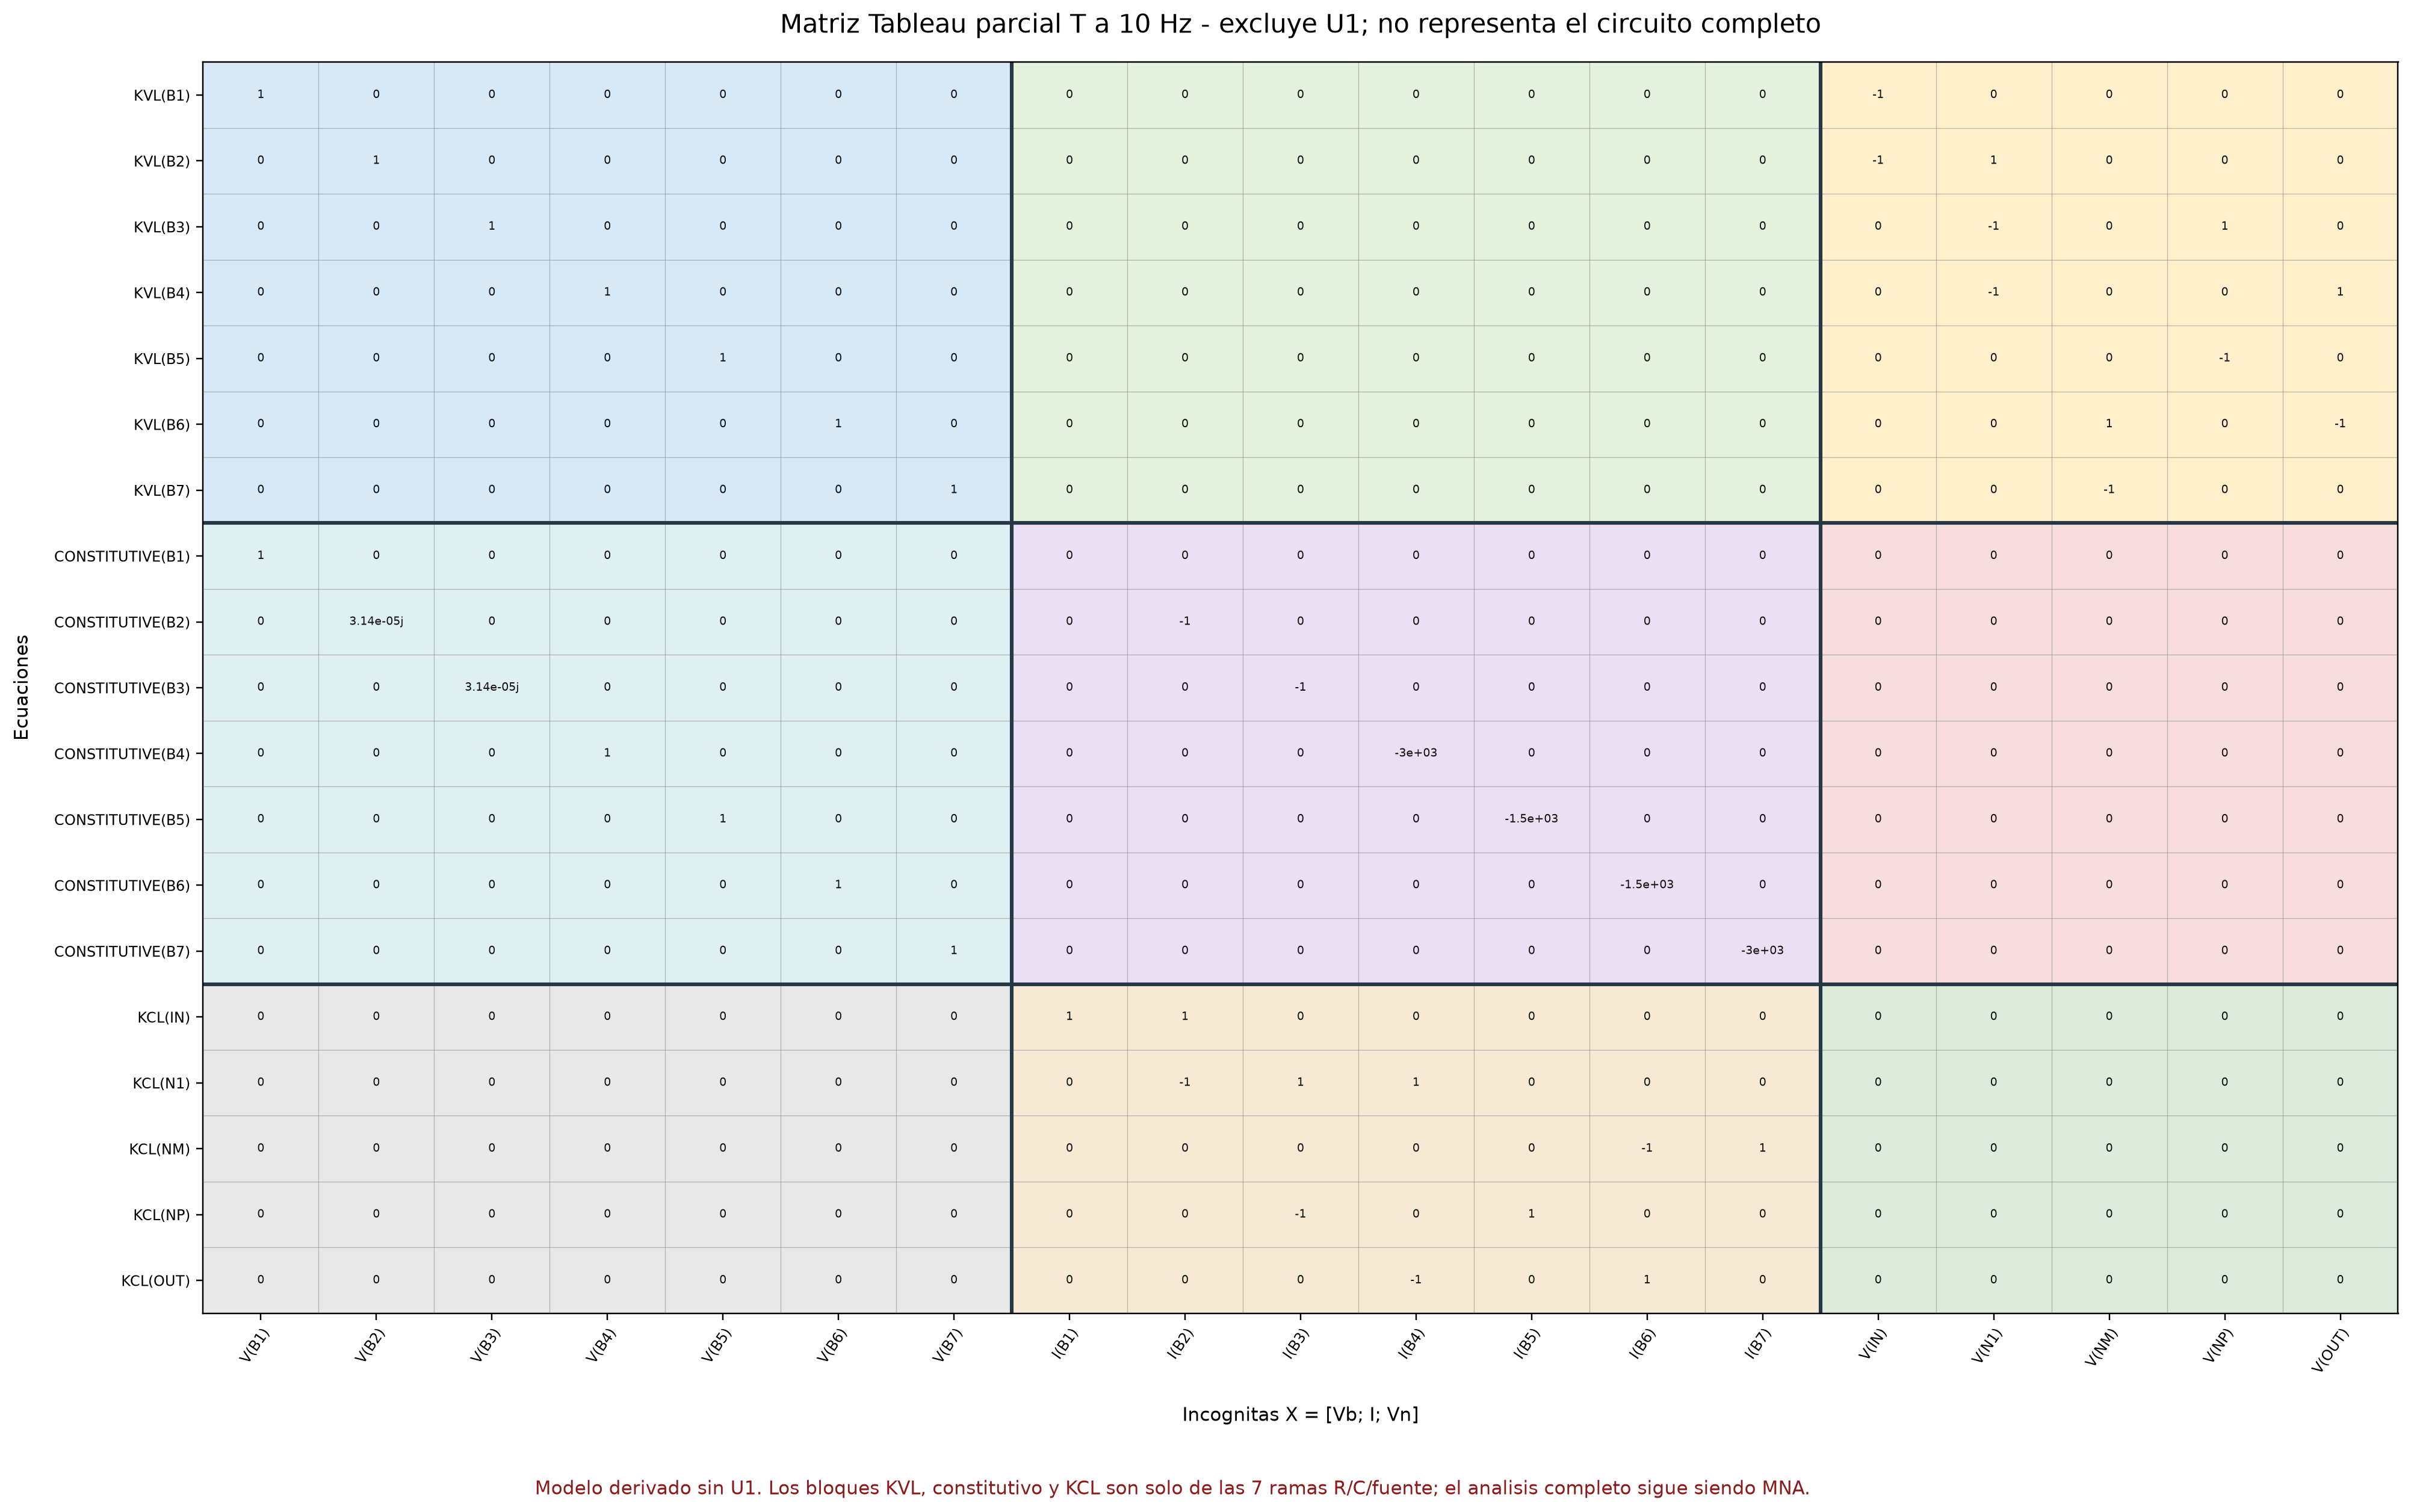
\includegraphics[width=0.9\linewidth]{2_circuito_objetivo_modificado_agent/plots/tableau_partial_T_colored_blocks_10Hz.png}
\caption{Matriz Tableau parcial a 10 Hz; excluye el op-amp ideal.}
\end{figure}

\begin{figure}[H]
\centering
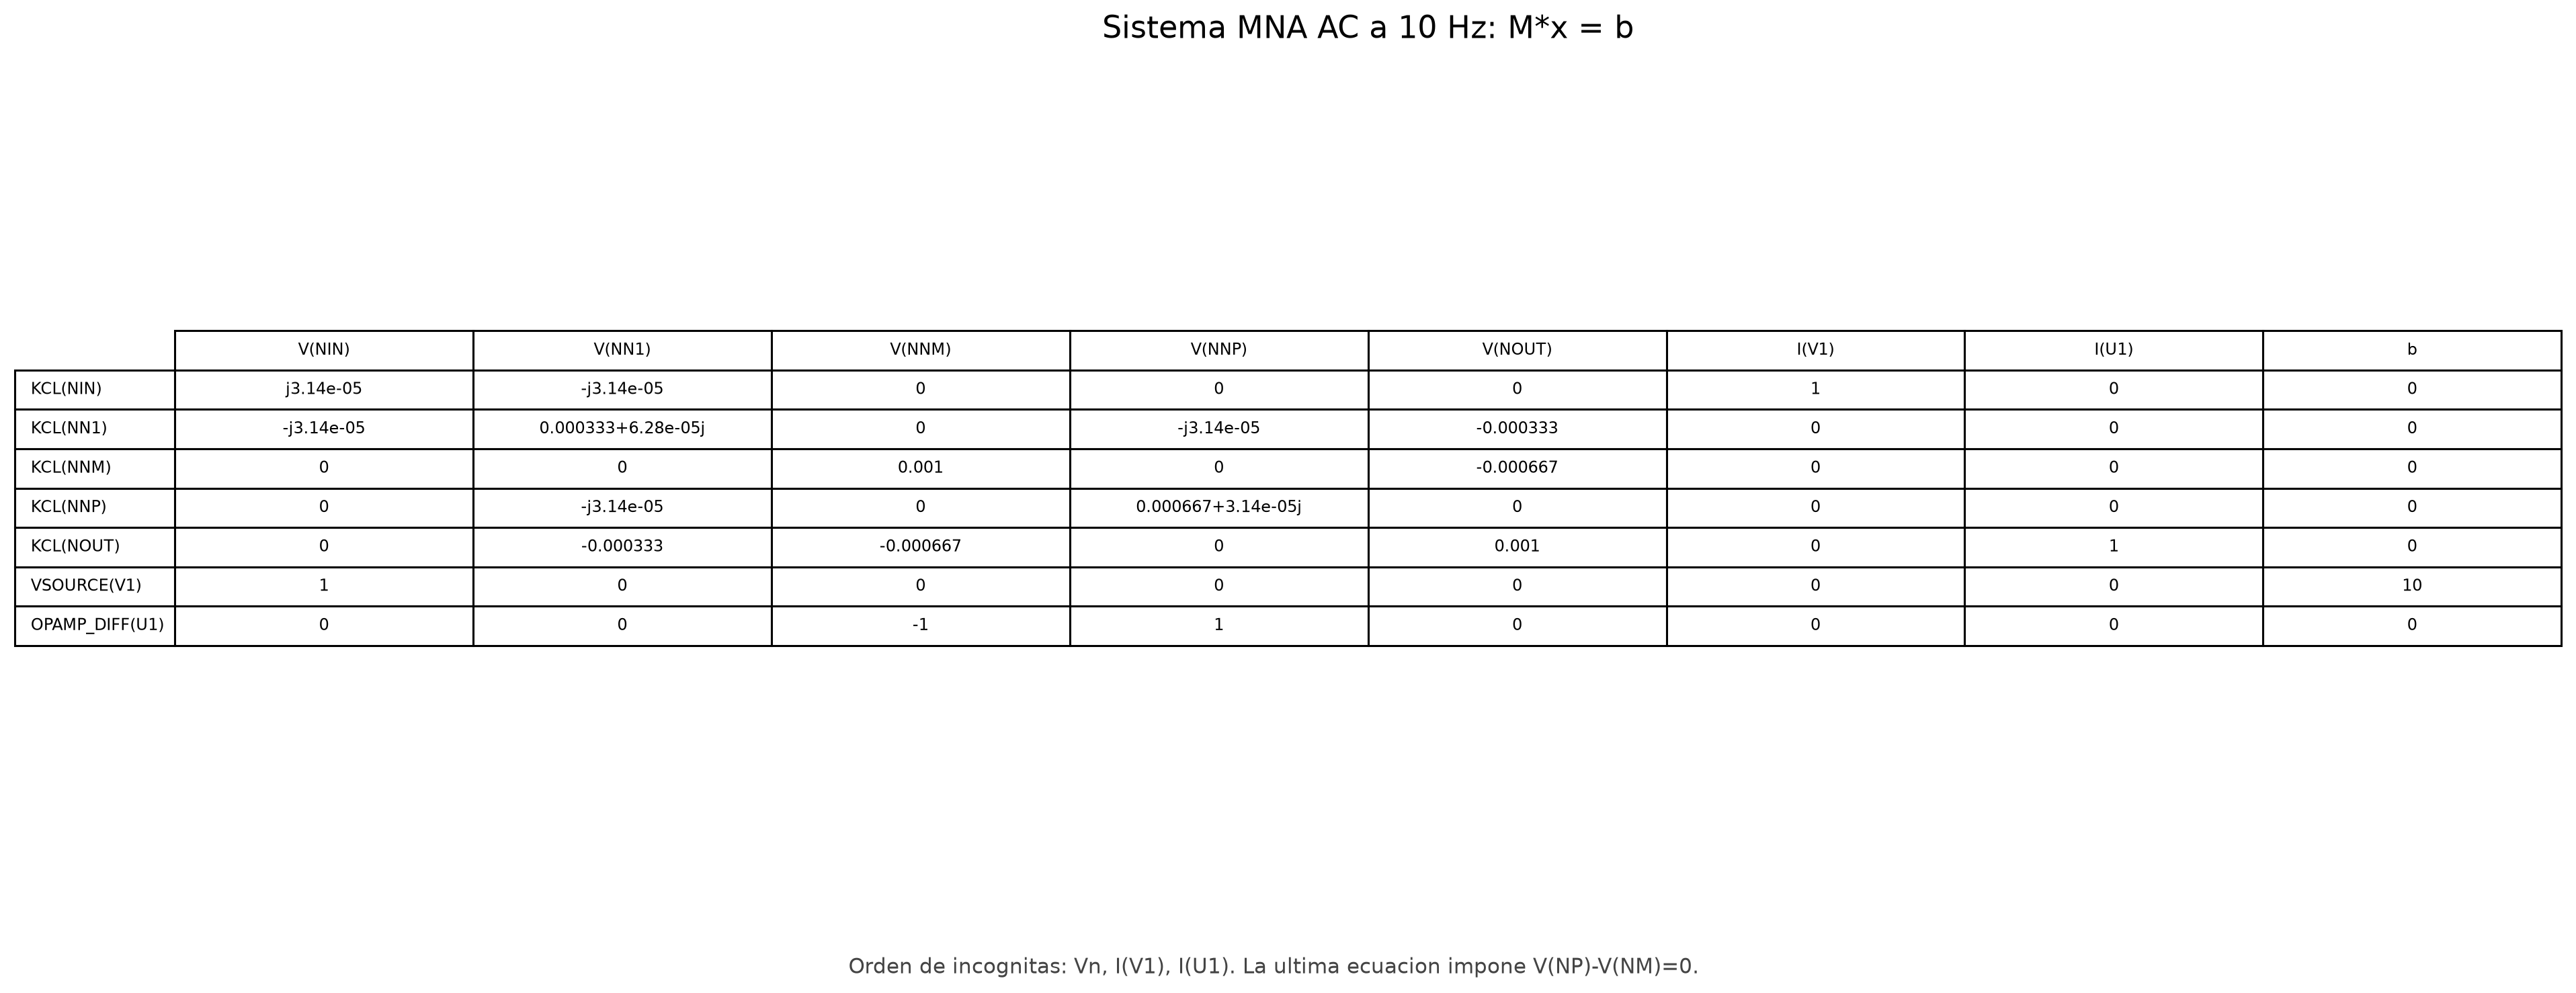
\includegraphics[width=0.95\linewidth]{../../filtro_activo_20261116_1710_circuito_objetivo_modificado/mna_system_10Hz.png}
\caption{Sistema MNA AC completo del circuito a 10 Hz.}
\end{figure}

\subsection{Resultados del analisis en AC del Agente y HSPICE}
Para documentar la transferencia se ejecutó el barrido MNA de 300 puntos sobre los artefactos normalizados de esta ejecución, solicitando explícitamente $H(w)=V(OUT)/V(IN)$. El barrido adicional reportó estado global \textbf{Satisfactorio}. Los valores de la tabla proceden del agente SPICE.

\begin{table}[H]
\centering
\begin{tabular}{lrrr}
\toprule
Punto & Frecuencia (Hz) & $H(w)$ (dB) & Fase ($^\circ$) \\
\midrule
Inicio & 10 & -43.6069 & 170.5933 \\
Fin & 100000 & 3.5218 & 0.2128 \\
\bottomrule
\end{tabular}
\caption{Valores representativos de la transferencia del circuito modificado.}
\end{table}

La magnitud de voltaje de salida informada directamente por el agente SPICE fue 0.0660172 V a 10 Hz y 14.99993 V a 100 kHz. Las figuras presentan la magnitud de transferencia, el voltaje de salida y la fase.

\begin{figure}[H]
\centering
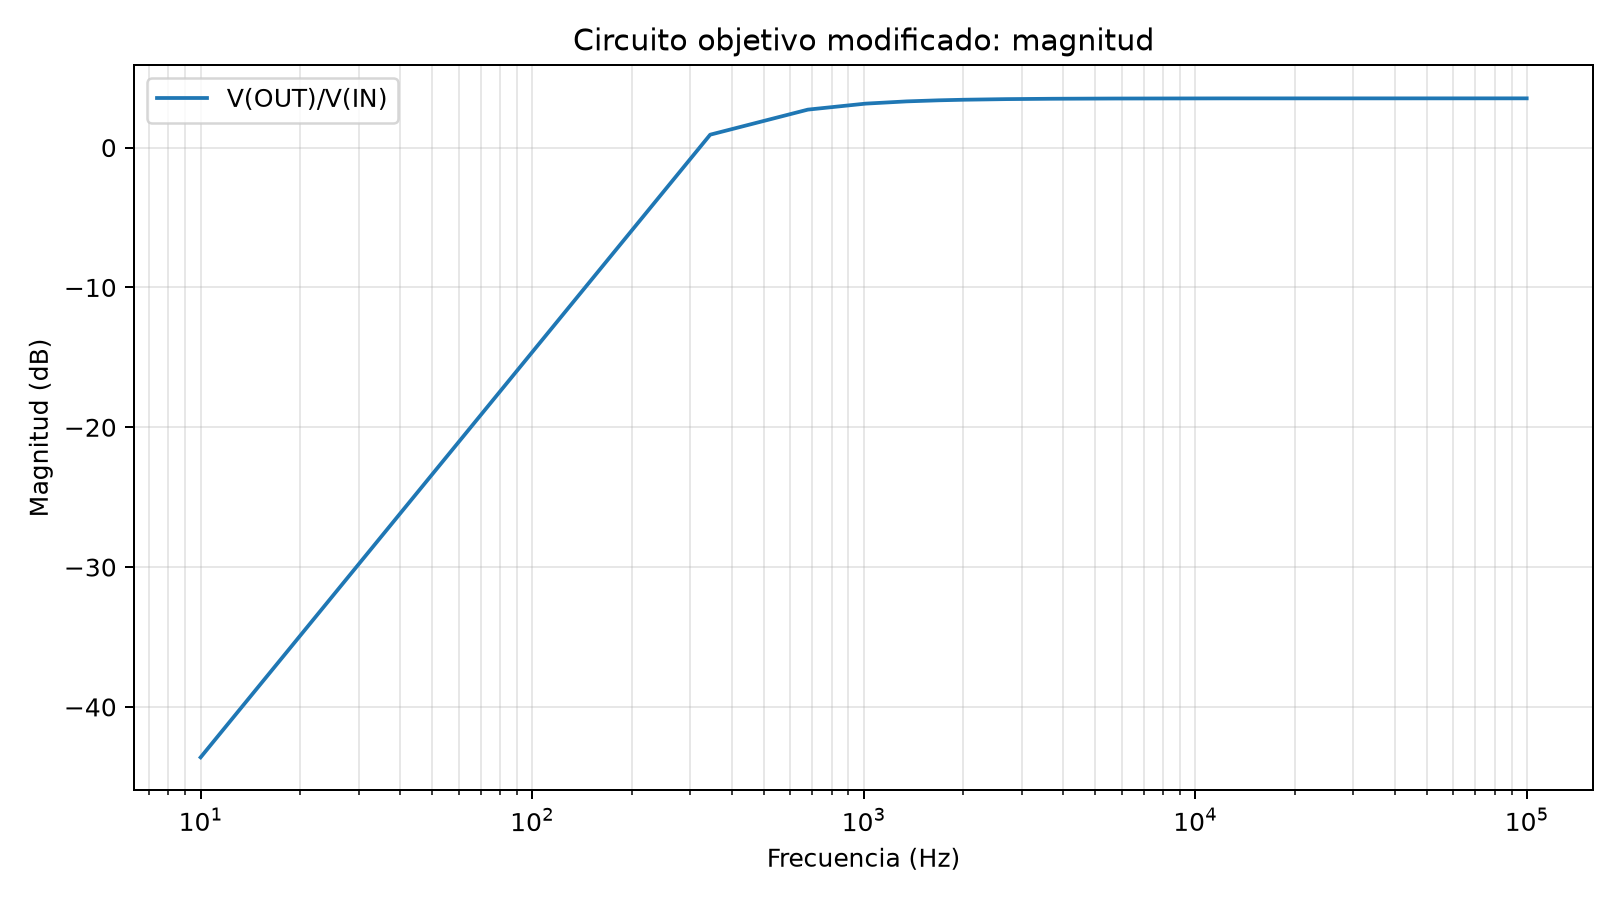
\includegraphics[width=0.78\linewidth]{../comparaciones_20261117_1306/caso2_plots/magnitude.png}
\caption{Gráfica de Magnitud en dB de la función de transferencia $H(w)$ obtenida por el agente.}
\end{figure}

\begin{figure}[H]
\centering
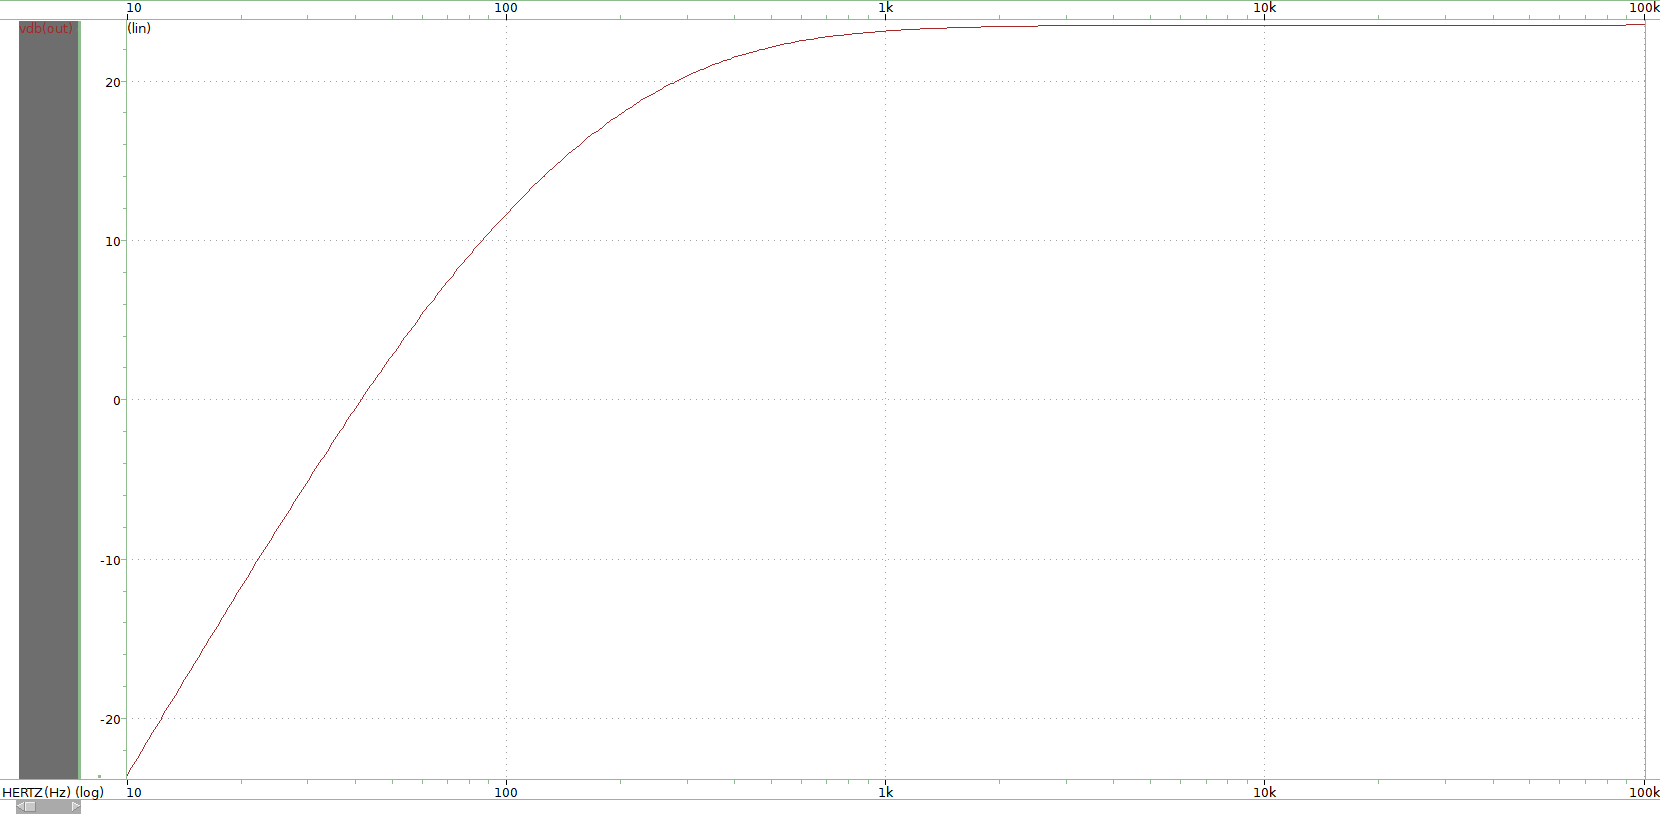
\includegraphics[width=0.78\linewidth]{2_circuito_objetivo_modificado_HSPICE/magnitude_dB.png}
\caption{Gráfica de Magnitud en dB de la función de transferencia $H(w)$ obtenida por HSPICE.}
\end{figure}

\begin{figure}[H]
\centering
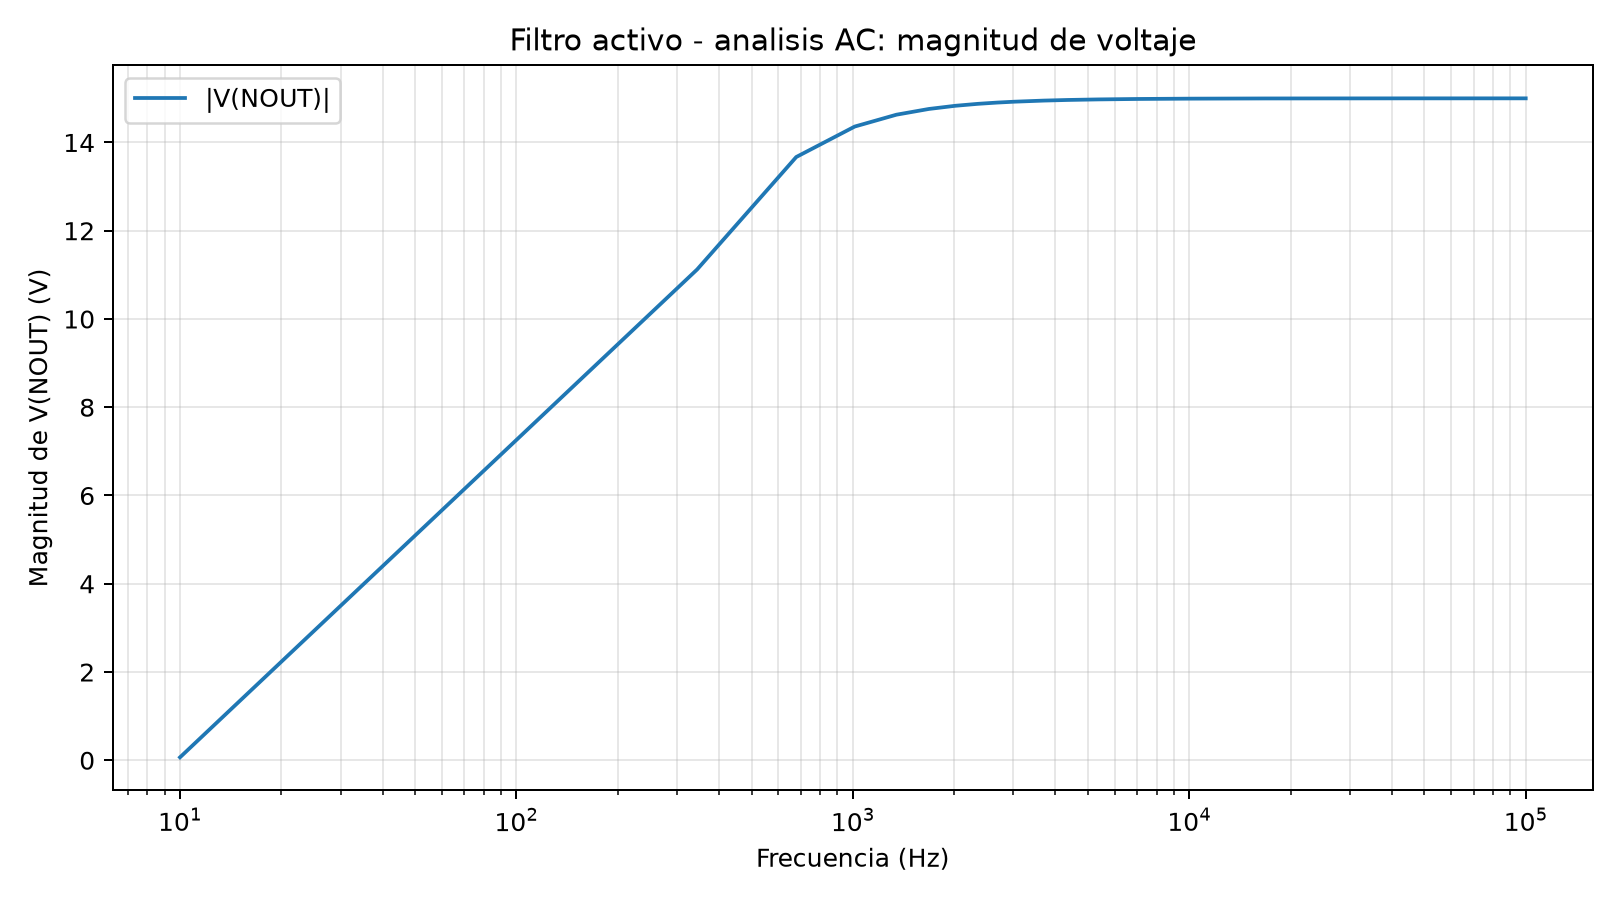
\includegraphics[width=0.78\linewidth]{2_circuito_objetivo_modificado_agent/plots/magnitude_voltage.png}
\caption{Gráfica de Magnitud en Voltaje de $V\_OUT$ obtenida por el agente.}
\end{figure}

\begin{figure}[H]
\centering
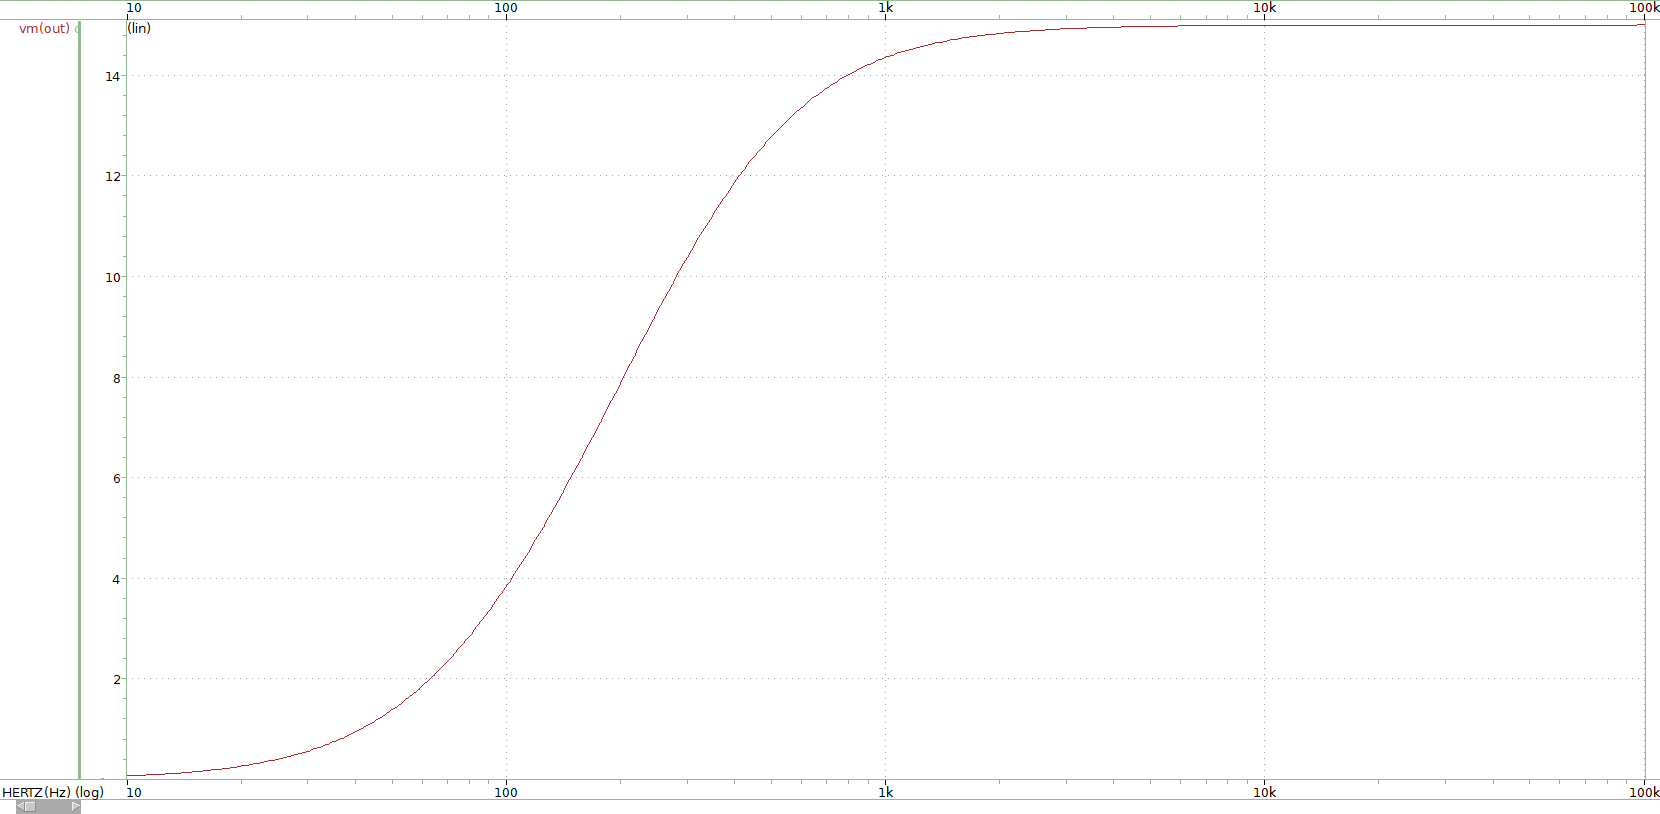
\includegraphics[width=0.78\linewidth]{2_circuito_objetivo_modificado_HSPICE/magnitude_voltage.png}
\caption{Gráfica de Magnitud en Voltaje de $V\_OUT$ obtenida por HSPICE.}
\end{figure}

\begin{figure}[H]
\centering
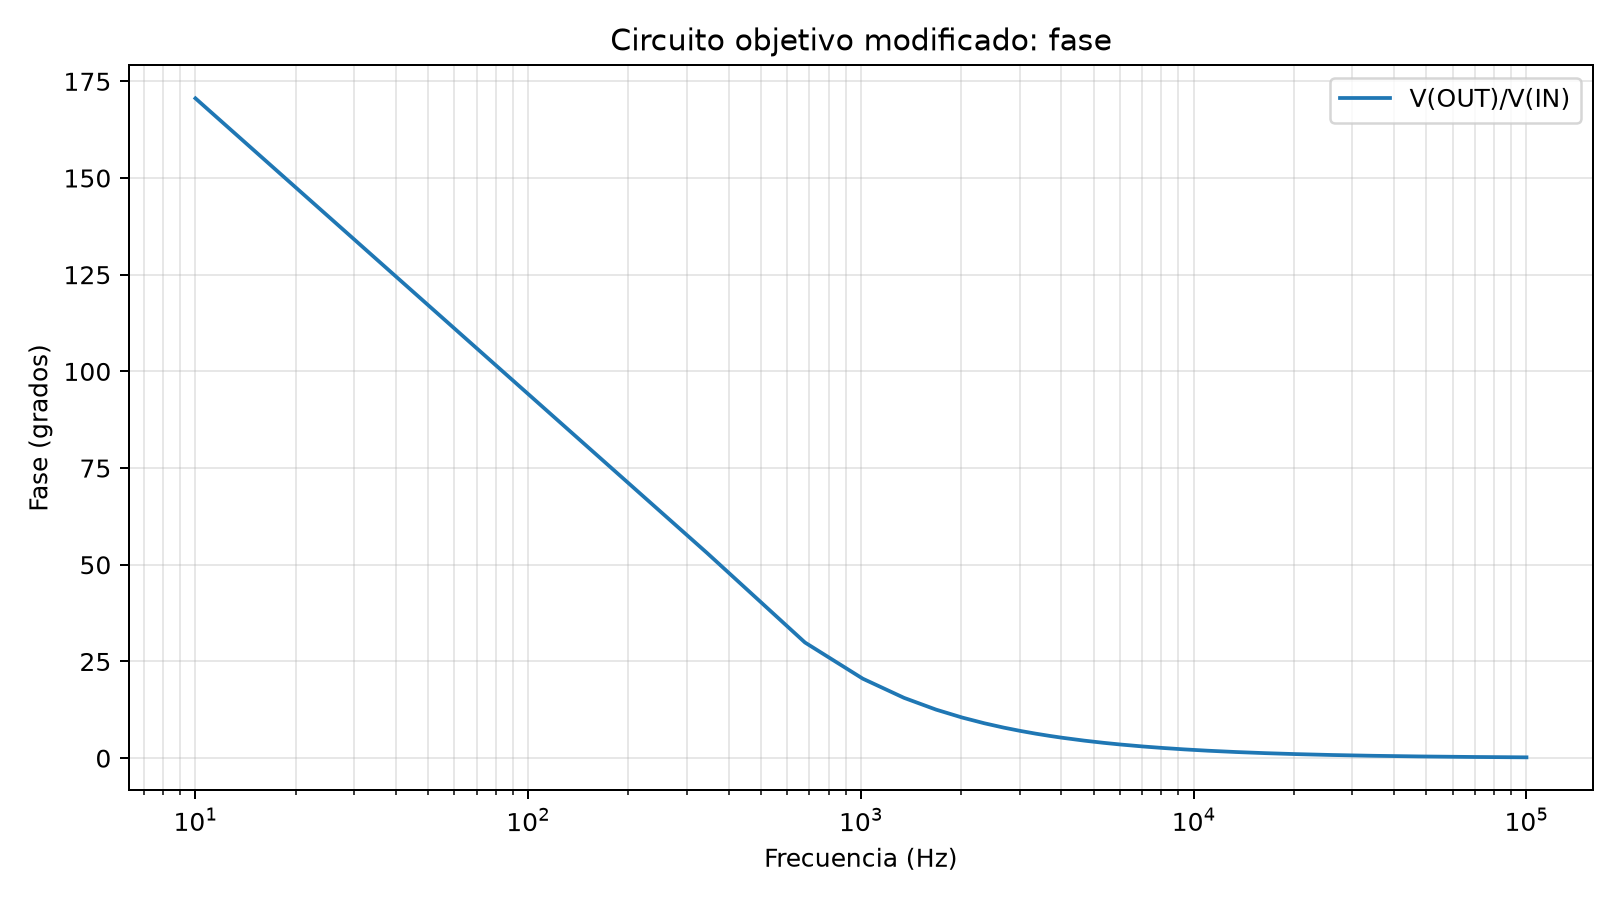
\includegraphics[width=0.78\linewidth]{../comparaciones_20261117_1306/caso2_plots/phase.png}
\caption{Gráfica de Fase de la función de transferencia $H(w)$ obtenida por el agente.}
\end{figure}


\begin{figure}[H]
\centering
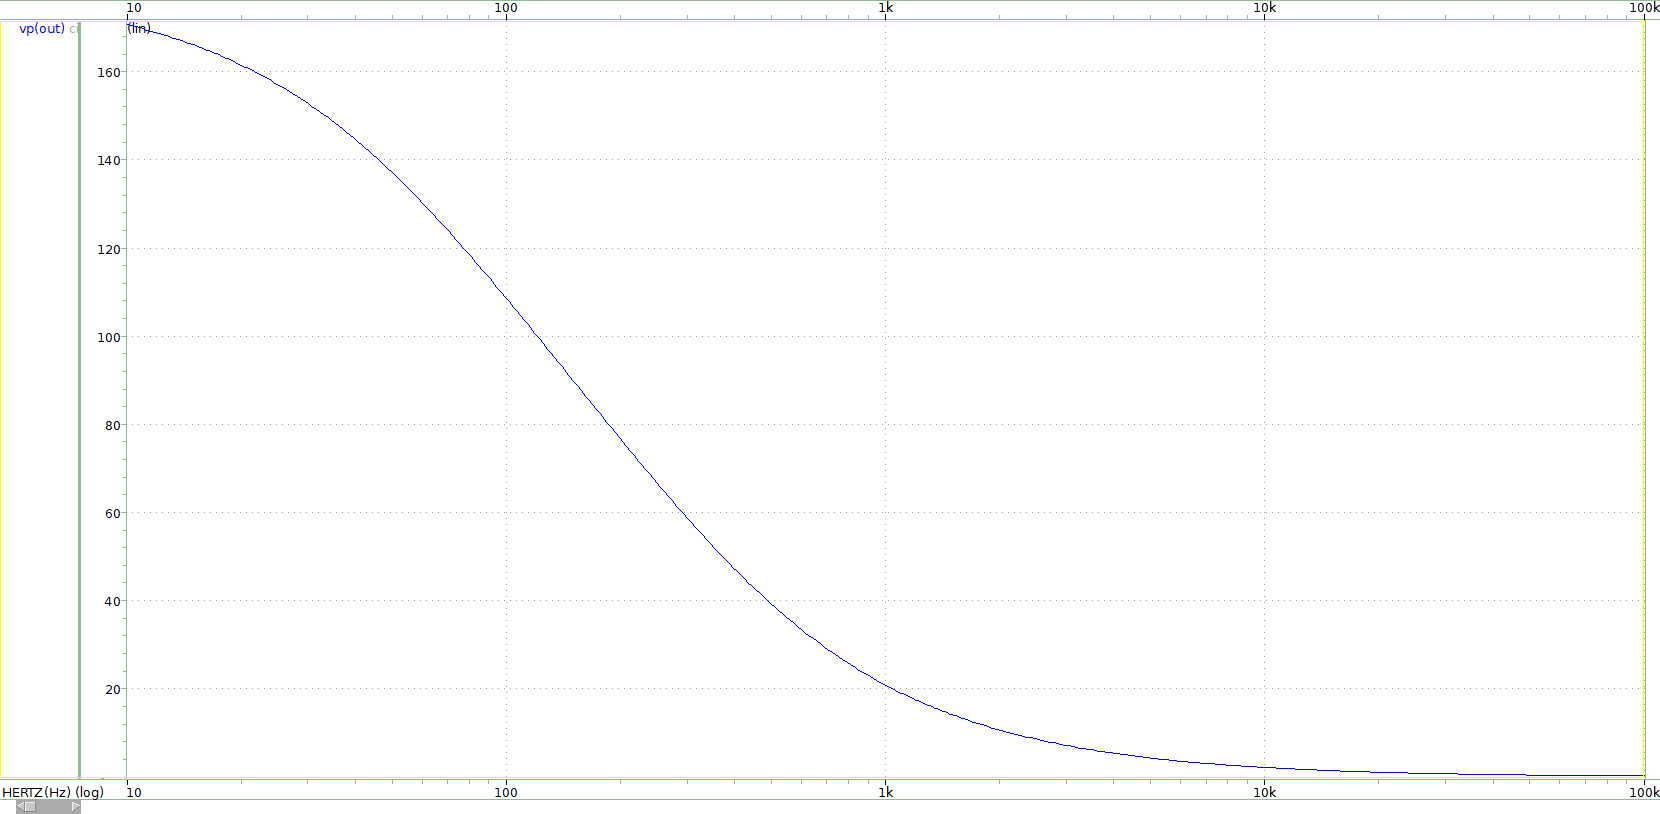
\includegraphics[width=0.78\linewidth]{2_circuito_objetivo_modificado_HSPICE/phase.png}
\caption{Gráfica de Fase de la función de transferencia $H(w)$ obtenida por HSPICE.}
\end{figure}


\subsection{Comparación con HSPICE}
La referencia corresponde a los datos obtenidos por HSPICE. HSPICE usó 401 puntos DEC entre 10 Hz y 100 kHz, mientras que el agente usó 300 puntos LIN; por ello se compararon únicamente las dos frecuencias exactamente coincidentes, sin interpolación. Ambos circuitos usan una entrada AC de 10 V. La referencia aproxima el op-amp con una fuente dependiente de ganancia finita $10^9$, mientras que el agente emplea el modelo ideal MNA; por tanto, el acuerdo en los extremos no implica equivalencia de modelos ni valida todos los puntos del barrido.

La herramienta \texttt{compare\_reference.py} comparó los fasores de salida $V(NOUT)$ con tolerancias absoluta $10^{-6}$ V y relativa $2\times10^{-5}$. Los fasores, errores y estados siguientes proceden de su artefacto de comparación.

\begin{table}[H]
\centering
\small
\begin{tabularx}{\linewidth}{lXX}
\toprule
Frecuencia & Agente MNA: $V(NOUT)$ (V) & HSPICE: $V(OUT)$ (V) \\
\midrule
10 Hz & $-6.51294636\times10^{-2}+j1.07899595\times10^{-2}$ & $-6.51294704\times10^{-2}+j1.07899388\times10^{-2}$ \\
100 kHz & $14.99982691+j5.57037127\times10^{-2}$ & $14.99979657+j5.57036035\times10^{-2}$ \\
\bottomrule
\end{tabularx}
\caption{Fasores de salida en los puntos de frecuencia coincidentes.}
\end{table}

\begin{table}[H]
\centering
\begin{tabular}{lrrc}
\toprule
Frecuencia & Error absoluto (V) & Error relativo & Estado \\
\midrule
10 Hz & $2.1769\times10^{-8}$ & $3.2974\times10^{-7}$ & \textbf{PASS} \\
100 kHz & $3.0342\times10^{-5}$ & $2.0228\times10^{-6}$ & \textbf{PASS} \\
\bottomrule
\end{tabular}
\caption{Comparación compleja de voltajes de salida; resultado global \textbf{Satisfactorio} (2/2 puntos).}
\end{table}

La gráfica HSPICE $VDB(OUT)$ está en dBV (voltaje de salida), mientras que la gráfica del agente está en dB de $V(OUT)/V(IN)$; por la entrada de 10 V, estas magnitudes no tienen la misma referencia y no deben compararse directamente. La comparación cuantitativa se realiza con los fasores de salida en voltios y cubre únicamente los dos puntos coincidentes.


La comparación es reproducible con los artefactos JSON de puntos, referencia HSPICE y resultado de \texttt{compare\_reference.py}, conservados en la carpeta de comparación del reporte.